% !TeX spellcheck = pt_BR
 \documentclass[a4paper,12pt]{report}
\usepackage[a4paper,top=3cm,bottom=2cm,left=3cm,right=3cm,marginparwidth=1.75cm]{geometry}
\usepackage[brazil]{babel}
\usepackage[T1]{fontenc}
\usepackage[utf8]{inputenc}
\usepackage{amsmath}
\usepackage{amsthm}
\usepackage{MnSymbol}
\usepackage{wasysym}
\usepackage{hyperref}
\usepackage{color}
\definecolor{Blue}{rgb}{0,0,0.9}
\definecolor{Red}{rgb}{0.9,0,0}
\usepackage{esvect}
\usepackage{graphicx}
\usepackage{float}
\usepackage{indentfirst}
\usepackage{caption}
\usepackage{blkarray}
\newcommand\Mark[1]{\textsuperscript#1}
\usepackage{pgfplots}
\usepackage{amsfonts}
\usepackage[english, ruled, linesnumbered]{algorithm2e}
\usepackage{algorithmic}

\newcommand{\nucleoe}{\emph{\text{nu }}}
\newcommand{\nucleo}{\text{nu }}
\newcommand{\imageme}{\emph{\text{nu }}}
\newcommand{\imagem}{\text{nu }}

\theoremstyle{plain}
\newtheorem{teorema}{Teorema}[section]
\newtheorem{lema}{Lema}[section]
\newtheorem{proposicao}{Proposição}[section]
\newtheorem{corolario}{Corolário}[section]

\theoremstyle{definition}
\newtheorem{definicao}{Definição}[section]
\newtheorem{observacao}{Observação}[section]
\newtheorem{exemplo}{Exemplo}[section]

\newenvironment{solucao}
{\renewcommand\qedsymbol{$\triangle$}\begin{proof}[Solução]}{\end{proof}}

\title{Álgebra: notas de estudo}
\author{Guilherme Philippi}
\begin{document}
\maketitle
\tableofcontents

\chapter{Álgebra Abstrata}
% Enunciar as principais referências desse capítulo

\section{Relações entre conjuntos}

\begin{definicao}[Produto cartesiano]
	Sejam $A$ e $B$ conjuntos. O conjunto $$A\times B = \{(a,b) \ | \ a\in A \text{ e } b\in B\}$$
	é o \emph{produto cartesiano de A e B}.
\end{definicao}

\begin{exemplo}
	Se $A = \{1,2,3\}$ e $B = {3,4}$, então $$A\times B = \{(1,3),(1,4),(2,3),(2,4),(3,3),(3,4)\}.$$
\end{exemplo}

\begin{definicao}[Relação]
	Uma	\emph{relação} entre dois conjuntos $A$ e $B$ é um subconjunto $\mathcal{R}\subset A\times B$. Lê-se $(a,b) \in \mathcal{R}$ como ``$a$ está relacionado com $b$'' e escreve-se $a\mathcal{R}b$.
\end{definicao}

\begin{exemplo}[Relação de igualdade]\label{ex:igualdade}
	A realação $=$, chamada \emph{relação de igualdade}, é definida sobre um conjunto $S$ por $$= \text{é o subconjunto } \{(x,x) \ |\ x\in S\}\subset S\times S.$$
\end{exemplo}

\begin{observacao}
	Sempre que uma relação for definida entre um conjunto $S$ e ele mesmo, como no exemplo~\ref{ex:igualdade}, diremos que esta é uma relação \emph{sobre} $S$.
\end{observacao}

\begin{definicao}[Função]
		Uma \emph{função} $\varphi$ que mapeia $X$ em $Y$ é uma relação entre $X$ e $Y$ com a propriedade de que cada $x\in X$ só irá aparecer uma única vez, e exatamente uma, em um par ordenado $(x,y)\in \varphi$. Também chamamos $\varphi$ de \emph{mapa} ou \emph{mapeamento} de $X$ em $Y$. Escrevemos $\varphi: X\longrightarrow Y$ e expressaremos $(x,y)\in\varphi$ por $\varphi(x) = y$. O \emph{domínio} de $\varphi$ é o conjunto $X$ e o conjunto $Y$ é dito \emph{contradomínio} de $\varphi$. Chama-se de \emph{alcance} de $\varphi$ o conjunto $\varphi[X] = \{\varphi(x)\ | \ x \in X\}.$
\end{definicao}

\begin{definicao}[Função injetiva e sobrejetiva]
		Uma função $\varphi: X \longrightarrow Y$ é \emph{injetiva} se $\varphi(x_1) = \varphi(x_2) \iff x_1 = x_2$. Também, $\varphi$ é dita \emph{sobrejetiva} se o alcance de $\varphi$ é $Y$. Se uma função é injetiva e sobrejetiva, então dizemos que a função é \emph{bijetiva}.
\end{definicao}

\section{Lei de composição}

\begin{definicao}[Lei de composição]
	Uma \emph{lei de composição} sobre um conjunto \(S\) é uma função (ou, uma operação binária) \(*: S\times S \longrightarrow S\).
\end{definicao}

\begin{observacao}[Notação de operação]
	Usaremos a notação \(*(a,b) = a*b\), para simplificar a escrita de
	propriedades. Também, quando não houver ambiguidade, suprimiremos o simbolo da lei, fazendo $a*b = ab$.
\end{observacao}


\begin{definicao}
	Para $a,b,c \; \in S$, uma lei de composição $*$ é dita
	
	\begin{itemize}
		\item \emph{Associativa}, se $(a*b)*c = a*(b*c)$;
		\item \emph{Comutativa}, se \(a*b = b*a\).
	\end{itemize}
\end{definicao}

\begin{proposicao}
	Seja uma lei associativa dada sobre o conjunto
	\(S\). Há uma única forma de definir, para todo inteiro \(n\), um
	produto de \(n\) elementos \(a_1,\dots,a_n \in S\) (diremos
	\([a_1\dotsb a_n]\)) com as seguintes propriedades:
	
	\begin{enumerate}
		\def\labelenumi{\arabic{enumi}.}
		\item
		o produto \([a_1]\) de um elemento é o próprio elemento;
		\item
		o produto \([a_1a_2]\) de dois elementos é dado pela lei de
		composição;
		\item
		para todo inteiro \(1\leq i\leq n\),
		\([a_1\dotsb a_n] = [a_1\dotsb a_i][a_{i+1}\dotsb a_n]\).
	\end{enumerate}
\end{proposicao}

\begin{proof}
	A demonstração dessa proposição é feita por indução em \(n\).
\end{proof}

\begin{definicao}
	Dizemos que \(e\in S\) é \emph{identidade} para uma lei de composição se \(ea = ae = a\) para todo \(a\in S\).
\end{definicao}

\begin{proposicao}
	O elemento identidade é único.
\end{proposicao}
\begin{proof}
	Se \(e,e'\) são identidades, já que \(e\) é identidade, então \(ee' = e'\) e, como $e'$ é uma identidade, \(ee' = e\). Logo \(e = e'\), isto é, a identidade é única.
\end{proof}

\begin{observacao}
	Usaremos $\vec{1}$ para representar a identidade multiplicativa e $\vec{0}$ para denotar a aditiva.
\end{observacao}

\begin{definicao}[Elemento inverso]
	Seja uma lei de composição que possua uma identidade. Um elemento \(a\in S\) é chamado \emph{invertível} se há um outro elemento \(b\in S\) tal que \(ab = ba = 1\). Desde que \(b\) exista, ela é única e a denotaremos por \(a^{-1}\) e a chamaremos
	\emph{inversa de $a$}.
\end{definicao}


\begin{proposicao}
	Se \(a,b\in S\) possuem inversa, então a composição \((ab)^{-1} = b^{-1}a^{-1}\).
\end{proposicao}

\begin{observacao}[Potências]
	Usaremos as seguintes notações:
	\begin{itemize}
		\item \(a^n = a^{n-1}a\) é a composição de \(a\dotsb a\) \(n\) vezes;
		\item \(a^{-n}\) é a inversa de \(a^n\);
		\item \(a^0 = \vec{1}\).
	\end{itemize}

	Com isso, tem-se que \(a^{r+s} = a^ra^s\) e \((a^r)^s = a^{rs}\). (Isso
	não induz uma notação de fração \(\frac{b}{a}\) a menos que seja uma lei
	comutativa, visto que \(ba^{-1}\) pode ser diferente de \(a^{-1}b\)).
	Para falar de uma lei de composição aditiva, usaremos \(-a\) no lugar de
	\(a^{-1}\) e \(na\) no lugar de \(a^n\).
\end{observacao}

\section{Grupos}

\begin{definicao}[Grupo]
	
	Um \emph{grupo} $(G,*)$ é um conjunto \(G\) onde uma lei de
	composição $*$ é dada sobre \(G\) tal que os seguintes axiomas são satisfeitos:
	
	\begin{enumerate}
		\item \emph{(Associatividade).} Para todo $a,b,c \in G$, tem-se $$(a*b)*c = a*(b*c);$$
		\item \emph{(Existência da identidade).} Existe um elemento $\vec{1}\in G$ tal que, para todo $a\in G$, $$\vec{1}*a = a*\vec{1} = a;$$
		\item \emph{(Existência do inverso).} Para todo $a\in G$ existe um elemento $a'\in G$ tal que $$a*a' = a'*a = \vec{1}.$$
	\end{enumerate}
\end{definicao}

\begin{observacao}
	É comum abusar da notação e chamar um grupo $(G,*)$ e o conjunto de	seus elementos $G$ pelo mesmo simbolo, omitindo a lei de composição na falta de ambiguidade.	
\end{observacao}

\begin{definicao}[Grupo abeliano]
	Um \emph{grupo abeliano} é um grupo com uma lei de
	composição comutativa. Costuma-se usar a notação aditiva para grupos
	abelianos.
\end{definicao}

\begin{proposicao}[Lei do cancelamento]
	Seja \(a,b,c\) elementos de um grupo \(G\). Se \(ab = ac\), então \(b = c\).
\end{proposicao} 

\section{Subgrupos}

\begin{definicao}[Subgrupo]
	Um subconjunto \(H\) de um grupo \(G\) é chamado de \emph{subgrupo} de \(G\) (e escreve-se $H \leq G$) se possuir as seguintes propriedades:
	
	\begin{enumerate}
		\item \emph{(Fechado).} Se \(a,b\in H\), então \(ab\in H\);
		\item \emph{(Identidade).} \(1\in H\);
		\item \emph{(Inversível).} Se \(a\in H\), então \(a^{-1}\in H\).
	\end{enumerate}
	
\end{definicao}

\begin{observacao}[Lei de composição induzida]
	Veja que a propriedade 1 necessita de uma lei de composição. Usamos a
	lei de composição de \(G\) para definir uma lei de composição de \(H\),
	chamada \emph{lei de composição induzida}. Essas propriedades garantem
	que \(H\) é um grupo com respeito a sua lei induzida.
\end{observacao}

\begin{definicao}[Subgrupo apropriado]
	Todo grupo \(G\) possui dois subgrupos triviais: O subgrupo formado por
	todos os elementos de \(G\) e o subgrupo \(\{\vec{1}\}\), formado pela
	identidade de \(G\). Diz-se que um subgrupo é um \emph{subgrupo apropriado} se for diferente desses dois.
\end{definicao}

\begin{definicao}[Centro de um grupo]
	O \emph{centro} \(Z(G)\) de um grupo \(G\) é o
	conjunto de elementos que comutam com todo elemento de \(G\):
	\[Z(G) = \{z \in G \ | \ zx = xz \text{ para todo } x \in G\}.\]
\end{definicao}

\begin{exemplo}
	Utilizando da notação multiplicativa, define-se o
	\emph{subgrupo cíclico \(H\)} gerados por um elemento arbitrário \(x\)
	de um grupo \(G\) como o conjunto de todas as potências de \(x\):
	\(H = \{\dots , x^{-2}, x^{-1},\vec{1},x,x^2,\dots\}\).
\end{exemplo}

\begin{definicao}
	Chama-se \emph{ordem} de um grupo \(G\) o número \(|G|\) de elementos de \(G\).
\end{definicao}

Também pode-se definir um subgrupo de um grupo \emph{\(G\) gerado por um
subconjunto \(U \subset G\)}. Esse é o menor subgrupo de \(G\) que
contém \(U\) e consiste de todos os elementos de \(G\) que podem ser
espressos como um produto de uma cadeia de elementos de \(U\) e seus
inversos.

\begin{exemplo}
	O \emph{grupo de quaternions \(H\)} é o menor subgrupo
	do conjunto de matrizes \(2\times 2\) complexas invertíveis que não é
	cíclico. Isso consiste nas oito matrizes
	\[H = \{\pm 1, \pm \mathbf{i}, \pm \mathbf{j}, \pm \mathbf{k}\},\] onde
	
	\[
	1=
	\begin{bmatrix}
		1 & 0 \\
		0 & 1 \\
	\end{bmatrix},
	\ \mathbf{i}=
	\begin{bmatrix}
		i & 0 \\
		0 & -i \\
	\end{bmatrix},
	\ \mathbf{j}=
	\begin{bmatrix}
		0 & 1 \\
		-1 & 0 \\
	\end{bmatrix},
	\ \mathbf{k}=
	\begin{bmatrix}
		0 & i \\
		i & 0 \\
	\end{bmatrix}.
	\]
	
	Os dois elementos \(\mathbf{i}, \mathbf{j}\) geram \(H\), e o calculo
	leva as formulas
	
	\[\mathbf{i}^4 = 1, \quad \mathbf{i}^2 = \mathbf{j}^2, \quad \mathbf{j}\mathbf{i} = \mathbf{i}^3\mathbf{j}.\]
\end{exemplo}

\section{Homomorfismos}

\begin{definicao}[Homomorfismo de grupo]
	Sejam \((G,*)\) e \((G',\cdot)\) dois grupos. Um \emph{homomorfismo} \(\varphi: G\longrightarrow G'\) é um mapeamento tal que
	\begin{equation}\tag{propriedade de homomorfismo}
		\varphi(a*b) = \varphi(a)\cdot\varphi(b), \; \forall \; a,b\; \in G.
	\end{equation}
\end{definicao}

\begin{exemplo}[Inclusão]
	Seja \(H\) o subgrupo de um grupo \(G\). O homomorfismo \(i: H \longrightarrow G\) é dito \emph{inclusão} de \(H\) em \(G\), definido por \(i(x) = x\).
\end{exemplo}

\begin{proposicao}\label{prop:homo}
	 Um homomorfismo \(\varphi: G\longrightarrow G'\) mapeia a identidade de $G$ à identidade de $G'$ e transforma as inversas de $G$ nas respectivas inversas em $G'$. Isto é, as seguintes propriedades valem
	 \begin{itemize}
	 	\item \(\varphi(\vec{1}) = \vec{1}\) e 
	 	\item \(\varphi(a^{-1}) = \varphi(a)^{-1}\).	
 	 \end{itemize}
	  
\end{proposicao}

\begin{observacao}
	Por conta da Proposição~\ref{prop:homo}, dizemos que o mapeamento $\varphi$ \emph{preserva a estrutura algébrica de grupo}.
\end{observacao}

\begin{exemplo}
	Seja $\varphi: G \longrightarrow G'$ um homomorfismo de grupo sobrejetivo de $G$ em $G'$. Queremos mostrar que, se $G$ é abeliano, então $G'$ deve ser abeliano. Isto é, seja $a',b'\in G'$, queremos mostrar que $a'b' = b'a'$. Como $\varphi$ é sobrejetiva, existe $a,b\in G$ tal que $\varphi(a) = a'$ e $\varphi(b) = b'$. Pela propriedade de homomorfismo, $a'b' = \varphi(a)\varphi(b) = \varphi(ab)$ e, se $G$ é abeliano, $\varphi(ab) = \varphi(ba) = \varphi(b)\varphi(a) = b'a'$. Segue que $G'$ deve ser abeliano.
\end{exemplo}

\begin{definicao}[Imagem]
	A \emph{imagem} de um homomorfismo
	\(\varphi: G\longrightarrow G'\) é o subconjunto de \(G'\)	\[\text{im}\ \varphi = \{x\in G' \ |\ x = \varphi(a), \text{ para algum } a\in G\} = \varphi(G).\]
\end{definicao}

\begin{proposicao}
	A imagem de um homomorfismo $\varphi: G \longrightarrow G'$ é um subgrupo de $G'$.
\end{proposicao}

\begin{definicao}[Núcleo]
	O \emph{núcleo} do homomorfismo $\varphi: G \longrightarrow G'$ é o subconjunto de
	\(G\) formado pelos elementos que são mapeados pela identidade em
	\(G'\):	\[\text{nu} \ \varphi = \{a \in G \ | \ \varphi(a) = \vec{1}\} = \varphi^{-1}(\vec{1}).\]
\end{definicao}

\begin{proposicao}
	O núcleo de um homomorfismo $\varphi: G \longrightarrow G'$ é um subgrupo de $G$.
\end{proposicao}

\section{Isomorfismos}

\begin{definicao}[Isomorfismo de grupos]
	Dois grupos \((G,*)\) e \((G',\cdot)\) são ditos \emph{isomorfos} se possuírem um homomorfismo bijetivo entre si, isto é, há um mapeamento \emph{bijetivo} $\varphi: G \longrightarrow G'$ (chamado \emph{relação de isomorfismo}) que respeita a propriedade de homomorfismo:
	\[\varphi(a*b) = \varphi(a)\cdot\varphi(b) \text{, para todo } a,b \in G.\] 
\end{definicao}

\begin{observacao}
	Usa-se a notação $G \approx G'$ para dizer que $G$ é isomorfo a $G'$.  
\end{observacao}

\begin{definicao}[Classe de isomorfismo]
	Diz-se que o conjunto de grupos isomórfos a um dado grupo \(G\) é a \emph{classe de isomorfismo de \(G\)}.	
\end{definicao}

\begin{proposicao}
	Qualquer dois grupos em uma mesma classe de isomorfismo também são isomorfos entre si.
\end{proposicao}

\begin{definicao}[Automorfismo]
	Quando uma relação de isomorfismo \(\varphi: G\longrightarrow G\) é definida de um grupo \(G\) para ele mesmo,	chamamos esse tipo de isomorfismo de \emph{automorfismo} de \(G\).
\end{definicao}

\begin{exemplo}[Conjugação]
	 Seja \(b\in G\) um elemento fixo. Então, a
	\emph{conjugação de \(G\) por \(b\)} (também chamado \emph{automorfismo interno de $G$ por $g$}) é o mapeamento \(\varphi\) de \(G\)
	para ele mesmo definido por
	\[\varphi_b(x) = bxb^{-1}.\]
	Esse é um automorfismo porque:
	\begin{itemize}
		\item é compatível com a propriedade de homomorfismo: \[\varphi_b(xy) = bxyb^{-1} = bx\vec{1}yb^{-1} = bxb^{-1}byb^{-1} = \varphi_b(x)\varphi_b(y);\]
		\item é um mapa bijetivo visto que existe a função inversa $\varphi_b^{-1}(x) = b^{-1}xb = \varphi_{b^{-1}}(x)$ (isto é, a conjugação por \(b^{-1}\)) que, de forma análoga, também é compatível com a propriedade de homomorfismo.
	\end{itemize}
\end{exemplo}

\begin{observacao}[Abelianos]\label{ob:conjugadosDeAbelianos}
	Se o grupo é abeliano possui a conjugação trivial:
	\(bab^{ -1} = abb^{-1} = a\) (mapa identidade). Porém, qualquer grupo não comutativo tem alguma conjugação não trivial, isto é, existe ao menos um $b$ que não está no centro do grupo, portanto, ao menos o automorfismo não trivial dado pela conjugação do grupo por $b$ existe. 
\end{observacao}

\begin{definicao}[Conjugado]
	O elemento \(bab^{-1}\) é chamado \emph{conjugado de \(a\) por \(b\)}. Dois elementos \(a, a'\in G\) são ditos \emph{conjugados} se existe \(b\in G\) tal que \(a' = bab^{-1}\).	
\end{definicao}

\begin{observacao}
	O conjugado tem uma interpretação muito útil: Se escrevermos
	\(bab^{-1}\) como \(a'\), então \[ba = a'b.\] Ou seja, pode-se pensar na
	conjugação como a mudança em \(a\) que resulta de mover \(b\) de um lado
	para o outro na equação.
\end{observacao}		


\begin{proposicao}
	Seja $\varphi: G \longrightarrow G'$ um homomorfismo. Se \(a\in \nucleoe\varphi\) e \(b\) é qualquer elemento do grupo \(G\), então o conjugado \(bab^{-1} \in \nucleoe\varphi\).
\end{proposicao}

\begin{definicao}[Subgrupo normal]
	Um subgrupo \(N\) de um grupo \(G\) é chamado \emph{subgrupo normal} (escreve-se $N\trianglelefteq G$) se para cada \(a\in N\) e \(b\in G\), o conjugado
	\(bab^{-1} \in N\).
\end{definicao}

\begin{observacao}
	Fica claro que o núcleo de um homomorfismo é um subgrupo normal. Além disso, todo subgrupo de um grupo abeliano também é um subgrupo normal, porém, isso não é
	necessariamente verdade em subgrupos de grupos não abelianos (veja Observação~\ref{ob:conjugadosDeAbelianos}). 
\end{observacao}

\begin{proposicao}
	O centro de todo grupo é um subgrupo normal do grupo.
\end{proposicao}

\section{Grupos de Permutação}

\begin{definicao}[Permutação de um conjunto]
		Uma permutação de um conjunto $A$ é uma função bijetiva $\varphi: A \longrightarrow A$ do conjunto para ele mesmo.
\end{definicao}

\begin{proposicao}[Multiplicação de permutações]\label{def:multpermut}
	Seja $A$ um conjunto onde duas permutações $\tau,\sigma$ são dadas. A composição de funções $\tau\circ\sigma$ (chamada \emph{multiplicação de permutações}) é uma lei de composição sobre A.
\end{proposicao}

\begin{proposicao}
	Sejam $A$ um conjunto não vazio, $S_A$ o conjunto de todas as permutações de $A$ e $\circ$ uma multiplicação de permutações sobre $A$. Então, $(S_A, \circ)$ é um grupo.
\end{proposicao}

\begin{definicao}[Grupo simétrico sobre $n$ símbolos]
	Seja $A$ o conjunto finito $\{1,2,\dots, n\}$. O grupo de todas as permutações de $A$ é um \emph{grupo simétrico sobre os $n$ símbolos $1,2,\dots,n$} e é representado por $S_n$.	
\end{definicao}

\begin{observacao}
	É importante perceber que $S_n$ possui $n!$ elementos, isso é, a quantidade de toda combinação de $n$ elementos.
\end{observacao}

\begin{exemplo}[Grupos diedrais]
	O grupo $S_3$ de $3! = 6$ elementos forma um grupo de simetrias de um triangulo equilátero com vértices 1, 2 e 3. As 6 permutações que formam esse grupo são as 3 rotações e os 3 espelhamentos possíveis sobre os vértices do triangulo. Também chamamos $S_3$ de $D_3$, pois $D_3$ forma o terceiro \emph{grupo diedral}. 
	O $n$-ésimo grupo diedral $D_n$ é o grupo de simetrias de um polígono regular de $n$ vértices.
\end{exemplo}

\begin{definicao}[Restrição da imagem de uma função]
	Sejam $f: A\longrightarrow B$ uma função e $H$ um subconjunto de $A$. A \emph{imagem de $H$ por $f$} é $\{f(h)\ |\ h \in H\}$ e é representada por $f|_H$.
\end{definicao}

\begin{lema}
	Sejam $G$ e $G'$ grupos e $\varphi:G\longrightarrow G'$ um homomorfismo injetivo. Então, $\varphi|_G$ é um subgrupo de $G'$ e $\varphi$ provê um isomorfismo de $G$ com $\varphi|_G$.
\end{lema}

\begin{teorema}[Teorema de Cayley]
	Todo grupo é isomorfo a um grupo de permutações.
\end{teorema}

\section{Relações de Equivalência e Partições}

\begin{definicao}[Partições]
	Seja \(S\) um conjunto. Uma \emph{particão} \(P\) de
	\(S\) é uma subdivisão de \(S\) em subconjuntos não vazios e não
	sobrepostos, isto é, uma união de conjuntos disjuntos.	
\end{definicao}

\begin{exemplo}
	Pode-se particionar o conjunto dos números inteiros
	\(\mathbb{Z}\) na união de disjuntos \(P\cup I\), onde
	\(P = \{z \in \mathbb{Z} \ |\ z \text{ é par}\}\) e
	\(I = \{z \in \mathbb{Z} \ |\ z \text{ é impar}\}\).
\end{exemplo}

\begin{definicao}[Relações de equivalência]
	Uma \emph{relação de equivalência} sobre um conjunto
	\(S\) é uma relação que se mantém sobre um subconjunto de elementos de
	\(S\). Escreve-se \(a\sim b\) para representar a equivalência de
	\(a, b \in S\), que precisa respeitar os seguintes axiomas:
	\begin{enumerate}
		\item \emph{(Transitiva).} Se \(a\sim b\) e \(b\sim c\), então \(a\sim c\);
		\item \emph{(Simétrica).} Se \(a\sim b\), então \(b\sim a\);
		\item \emph{(Reflexiva).} \(a\sim a\).
	\end{enumerate}
\end{definicao}

\begin{observacao}
	A noção de partição em \(S\) e a relação de equivalência em \(S\) são
	lógicamente equivalentes: Dada uma partição \(P\) sobre \(S\), pode-se
	definir uma relação de equivalência \(R\) tal que, se \(a\) e \(b\)
	estão no mesmo subconjunto partição, então \(a\sim b\) e, dada uma
	relação de equivalência \(R\), podemos definir uma partição \(P\) tal
	que o subconjunto que contêm \(a\) é o conjunto de todos os elementos
	\(b\) onde \(a\sim b\). Esse subconjunto é chamado de \emph{classe de
		equivalência de \(a\)}
	\[C_a = \{b\in S \ | \ a\sim b\}\]
	e \(S\) é particionado em classes de equivalência.
\end{observacao}

\begin{proposicao}
	Sejam \(C_a\) e \(C_b\) duas classes de equivalência do conjunto \(S\). Se existe \(d\) tal que \(d\in C_a\) e \(d\in C_b\), então \(C_a = C_b\).
\end{proposicao}

\begin{observacao}[Representante]
	Seja um conjunto \(S\). Suponha que exista uma relação de equivalência
	ou uma partição sobre \(S\). Então, pode-se construir um novo conjunto
	\(\bar{S}\) formado pelas classes de equivalência ou os subconjuntos
	partições de \(S\). Essa construção induz uma notação muito útil: para
	\(a\in S\), a classe de equivalência de \(a\) ou o subconjunto partição
	que contém \(a\) serão denotados como o elemento
	\(\bar{a} \in \bar{S}\). Desta forma, a notação \(\bar{a} = \bar{b}\)
	significa que \(a \sim b\) e chamamos \(a,b \in S\) de
	\emph{representantes} das respectivas classes de equivalência
	\(\bar{a}, \bar{b} \in \bar{S}\).
\end{observacao}

\begin{definicao}[Equivalência induzida por aplicação]
	Seja um mapeamento \(\varphi: S \longrightarrow T\).
	Chama-se de \emph{relação de equivalência determinada por \(\varphi\)} a
	relação dada por \(\varphi(a) = \varphi(b) \Rightarrow a \sim b\). Além
	disso, para um elemento \(t\in T\), o subconjunto de
	\(\varphi^{-1}(t) = \{s \in S\ | \ \varphi(s) = t\}\) é dito
	\emph{imagem inversa de \(t\) por \(\varphi\)}.
\end{definicao}

\begin{proposicao}
	Seja um mapeamento \(\varphi: S \longrightarrow T\)
	e \(t \in T\) um elemento qualquer de \(T\). Se a imagem inversa
	\(\varphi^{-1}(t)\) é não vazia, então \(t \in \text{im}\ \varphi\) e
	\(\varphi^{-1}(t)\) forma uma classe de equivalência
	\(\bar{\varphi}\in \bar{S}\) através da relação determinada por
	\(\varphi\).	
\end{proposicao}

\begin{definicao}[Congruência]
	Seja \(\varphi: G\longrightarrow G'\) um
	homomorfismo. A relação de equivalência definida por \(\varphi\) é
	usualmente denotada por \(\equiv\) ao invés de \(\sim\) e a chamamos de
	\emph{congruência}:
	\[\varphi(a) = \varphi(b) \ \Rightarrow \ a \equiv b, \ \text{para }a,b \in G.\]	
\end{definicao}

\begin{proposicao}
	Seja \(\varphi: G\longrightarrow G'\) um
	homomorfismo e \(a,b \in G\). Então as seguintes afirmações são
	equivalentes:
	\begin{itemize}
		\item
		\(\varphi(a) = \varphi(b)\)
		\item
		\(b = an\), para algum \(n\in \text{nu} \ \varphi\)
		\item
		\(a^{-1}b \in \text{nu} \ \varphi\).
	\end{itemize}	
\end{proposicao}

\begin{definicao}[classe lateral em relação ao núcleo]
	Seja \(\varphi: G\longrightarrow G'\) um
	homomorfismo, \(a \in G\) e \(n\in\text{nu}\ \varphi\). O conjunto
	\[a\text{ nu }\varphi = \{g\in G \ | \ g = an \text{, para algum } n\in\text{nu }\varphi\}\] é dito \emph{classe lateral de \(\text{nu }\varphi\) em \(G\)}.	
\end{definicao}

\begin{observacao}
	Pode-se particionar o grupo \(G\) em \emph{classes de congruência},
	formadas pelas classes laterais \(a\text{ nu }\varphi\). Estas são imagens
	inversas do mapeamento \(\varphi\).
\end{observacao}

\begin{proposicao}
	O homomorfismo de grupo
	\(\varphi: G\longrightarrow G'\) é injetivo se, e somente se, seu núcleo
	é o subgrupo trivial \(\{\vec 1\}\).
\end{proposicao}

\begin{observacao}
	Esse resultado da uma forma de verificar se um homomorfismo \(\varphi\)
	é também um isomorfismo: Se \(\text{nu }\varphi = \{1\}\) e
	\(\text{im } \varphi = G'\), então \(\varphi\) é, pelos respectivos
	motivos, injetiva e sobrejetiva. Então é um isomorfismo.
\end{observacao}

\section{Orbitas, ciclos e grupos alternados}

\begin{definicao}[Órbita]\label{def:orbit}
	Seja $\sigma$ uma permutação de um conjunto $A$. Chamamos de \emph{órbitas de $\sigma$} a classe de equivalência em $A$ determinada pela relação de equivalência $\sim$:
	$$\text{para }a,b \in A,\ a\sim b \iff b=\sigma^n(a), \text{ para algum }n\in\mathbb{Z}.$$
\end{definicao}

\begin{observacao}
	A relação apresentada na Definição~\ref{def:orbit} é, de fato, uma relação de equivalência. Como segue:
	\begin{itemize}
		\item é reflexiva, já que $a = \sigma^0(a) \implies a\sim a$;
		\item é simétrica pois, se $a\sim b \implies \exists\  n\in \mathbb{Z}$ tal que $b = \sigma^n(a)$, então $a = \sigma^{-n}(b)$. Como $-n\in\mathbb{Z}$, então $b\sim a$;
		\item é transitiva, visto que $a\sim b \implies b=\sigma^n(a)$ e $b \sim c \implies c = \sigma^m(b)$, para algum $n,m\in\mathbb{Z}$, então $c=\sigma^m(\sigma^n(a)) = \sigma^{m+n}(a) \implies a\sim c$.
	\end{itemize}
\end{observacao}

\begin{exemplo}[Órbita trivial]
	Já que a permutação identidade $i$ de $A$ leva cada elemento de $A$ para a mesma posição, as órbitas de $i$ são os subconjuntos de apenas um elemento de $A$.
\end{exemplo}

\begin{definicao}[Ciclo]
	Uma permutação $\sigma\in S_n$ é um \emph{ciclo} se possuir no máximo uma órbita contendo mais que um elemento. O \emph{comprimento} de um ciclo é o número de elementos de sua maior órbita.
\end{definicao}

\begin{exemplo}
	Seja a permutação 
	$$
	\begin{pmatrix}
		1 & 2 & 3 & 4 & 5 & 6 & 7 & 8\\
		\downarrow & \downarrow & \downarrow & \downarrow & \downarrow & \downarrow & \downarrow & \downarrow\\
		3 & 2 & 6 & 4 & 5 & 1 & 7 & 8
	\end{pmatrix}
	$$
	Como a órbita $(1,3,6)$ é a única que contém mais de um elemento, essa permutação sobre o conjunto $\{1,2,3,4,5,6,7,8\}$ é um ciclo de comprimento 3.
\end{exemplo}

\begin{observacao}[Notação de ciclos]
	Podemos representar um ciclo com a notação de uma única linha, da forma $$\mu = (1,3,6),$$ indicando apenas os elementos da maior órbita do ciclo. Perceba que as demais órbitas não precisam ser representadas pois serão os índices fixos da permutação.
\end{observacao}

\begin{exemplo}[Produto de ciclos]
	Pode-se construir uma permutação como um multiplicação de ciclos (veja a definição~\ref{def:multpermut}). Por exemplo,
	
	$$
	\sigma = 
	\begin{pmatrix}
		1 & 2 & 3 & 4 & 5 & 6 & 7 & 8\\
		\downarrow & \downarrow & \downarrow & \downarrow & \downarrow & \downarrow & \downarrow & \downarrow\\
		3 & 8 & 6 & 7 & 4 & 1 & 5 & 2
	\end{pmatrix}
	= (1,3,6)(2,8)(4,7,5).
	$$
\end{exemplo}

\begin{proposicao}
	Toda permutação $\sigma$ de um conjunto finito é um produto de ciclos disjuntos.
\end{proposicao}

\begin{definicao}[Transposição]
	Um ciclo de comprimento 2 é uma transposição.
\end{definicao}

\begin{corolario}
	Qualquer permutação de um conjunto finito de pelo menos dois elementos é um produto de transposições.	
\end{corolario}

\begin{definicao}[Permutações pares e impares]
	Uma permutação de um conjunto finito é \emph{par} ou \emph{impar} se pode ser expressa, respectivamente, por um número par ou impar de produtos de transposições.
\end{definicao}

\begin{proposicao}
	Uma permutação em $S_n$ pode ser expressa como um produto de um número impar de transposições se e somente se não puder ser expressa como um número par de transposições e vice-versa.
\end{proposicao}

\begin{proposicao}
	Seja o grupo simétrico $S_n$ com $n\geq 2$. Então, a coleção de todas as permutações impares de $\{1,2,\dots,n\}$ forma um subgrupo de $S_n$ de ordem $\frac{n!}{2}$.	
\end{proposicao}

\begin{definicao}[Grupo alternado]
	O subgrupo de $S_n$ formado pelas permutações impares de $n$ símbolos é chamado \emph{grupo alternado $A_n$}.
\end{definicao}

\begin{observacao}
	Os grupos $S_n$ e $A_n$ são muito importantes. O teorema de Cayley mostra que todo grupo finito $G$ é estruturalmente idêntico a algum subgrupo de $S_n$, para $n = |G|$. Pode-se mostrar que não há formulas envolvendo apenas radicais para solucionar uma equação polinomial de grau $n\geq 5$. Por mais que isso não seja óbvio, esse fato se deve, na verdade, a estrutura de $A_n$.
\end{observacao}


\section{Classe lateral}

Definimos classe lateral somente em relação ao núcleo de um homomorfismo mas,
na verdade, pode-se definir uma classe lateral para qualquer subgrupo \(H\) de
um grupo \(G\).

\begin{definicao}[classe lateral a esquerda]
	Seja um subgrupo \(H\) de um grupo \(G\). O
	subconjunto da forma \[aH = \{ah \ | \ h\in H\}\] é dito \emph{classe lateral a esquerda de \(H\) em \(G\)}.
\end{definicao}

\begin{proposicao}
	A classe lateral é uma classe de equivalência para a
	relação de congruência
	\[b = ah \Rightarrow a \equiv b, \text{ para algum } h\in H.\]	
\end{proposicao}

\begin{observacao}
	Daí segue que, como classes de equivalência particionam um grupo,
	classes laterais a esquerda de um subgrupo particionam o grupo.
\end{observacao}

\begin{definicao}[Índice de um subgrupo]
	O número de classes laterais a esquerda de um subgrupo
	\(H\) em um grupo \(G\) chama-se \emph{índice de \(H\) em \(G\)} e é
	denotado como \([G:H]\).	
\end{definicao}

\begin{observacao}
	Como há uma bijeção do subgrupo \(H\) para a classe lateral \(aH\), a
	cardinalidade de \(aH\) tem de ser a mesma de \(H\). Isto é, as
	classes laterais de \(H\) particionam \(G\) em partes de mesma ordem.
\end{observacao}

\begin{proposicao}
	Seja \(aH\) a classe lateral do subgrupo \(H\) no grupo
	\(G\). Então, a ordem \(|G|\) do grupo \(G\) é dada por
	\[|G| = |H|[G:H].\]	
\end{proposicao}

\begin{proposicao}[Teorema de Lagrange]
	Seja \(G\) um grupo finito e
	\(H\) um subgrupo de \(G\). A ordem de \(H\) divide a ordem de \(G\).
\end{proposicao}

\begin{definicao}[Ordem de um elemento]
	Seja \(G\) um grupo. A \emph{ordem de um elemento \(a\in G\)} é a ordem do grupo cíclico gerado por \(a\).	
\end{definicao}

\begin{proposicao}
	Seja um grupo \(G\) com \(p\) elementos tal que
	\(p\) é primo e \(a\in G\) diferente da identidade. Então \(G\) é o
	grupo cíclico \(\{1,a,\dots,a^{p-1}\}\) gerado por \(a\).
\end{proposicao}

\begin{observacao}
	Também podemos obter uma expressão para calcular a ordem de um grupo de
	homomorfismo. Seja \(\varphi: G\longrightarrow G'\) um homomorfismo.
	Como as classes laterais a esquerda do núcleo de \(\varphi\) são as imagens
	inversas \(\varphi^{-1}\), elas estão em uma correspondência biunívoca
	com a imagem. Daí segue que
	\[[G:\text{ nu }\varphi\ ] = |\text{ im }\varphi\ |.\]
\end{observacao}

\begin{proposicao}
	Seja \(\varphi: G\longrightarrow G'\) um
	homomorfismo onde \(G\) e \(G'\) são finitos. Então
	\[|G| = |\text{ nu }\varphi\ |\cdot|\text{ im }\varphi\ |.\]	
\end{proposicao}

\begin{definicao}[classes laterais a direita]
	Os conjuntos da forma
	\[Ha = \{ha \ | \ h \in H\}\] chamam-se \emph{classes laterais a direita de um
		subgrupo \(H\)}. Esses são classes de equivalência para a relação de
	congruência a direita
	\[b = ha \Rightarrow a \equiv b, \text{ para algum }h \in H.\]	
\end{definicao}

\begin{proposicao}
	Seja um subgrupo \(H\) de um grupo \(G\). As
	seguintes afirmações são equivalentes:
	
	\begin{itemize}
		\item
		\(H\) é subgrupo normal,
		\item
		\(aH = Ha\) para todo \(a\in G\).
	\end{itemize}	
\end{proposicao}

\section{Restrição de um homomorfismo para um subgrupo}

\begin{observacao}
	O objetivo dessa seção é apresentar ferramentas para analisar um subgrupo \(H\)
	do grupo \(G\) a fim de garantir propriedades do grupo \(G\). No geral,
	os subgrupos são mais específicos e menos complexos de se trabalhar.
\end{observacao}

\begin{proposicao}
	Sejam \(K\) e \(H\) dois subgrupos do grupo \(G\)
	tal que a interseção \(K\cap H\) é um subgrupo de \(H\). Se \(K\) é um
	subgrupo normal de \(G\), então \(K\cap H\) é um subgrupo normal de
	\(H\).	
\end{proposicao}

\begin{exemplo}
	Com esse resultado, se \(G\) é finito pode-se utilizar o
	Teorema de Lagrange para obter informações sobre a interseção dos dois
	subgrupos: a interseção divide \(|H|\) e \(|K|\). Se \(|H|\) e \(|K|\)
	não tem o mesmo fator de divisão, então \(K\cap H = \{1\}\).	
\end{exemplo}

\begin{definicao}[Restrição de um homomorfismo para um subgrupo]
	Sejam o homomorfismo \(\varphi:G\longrightarrow G'\)
	e \(H\) um subgrupo de \(G\). Uma \emph{restrição de \(\varphi\) para o subgrupo \(H\)} é o homomorfismo \(\varphi|_H:H\longrightarrow G'\)
	definido como
	\[\varphi|_H(h) = \varphi(h), \text{ para todo }h\in H.\]	
\end{definicao}

\begin{proposicao}
	Sejam o homomorfismo
	\(\varphi:G\longrightarrow G'\) e \(H\) um subgrupo de \(G\). O núcleo
	de uma restrição \(\varphi|_H\) é a interseção do núcleo de \(\varphi\)
	e \(H\).	
\end{proposicao}

\begin{proposicao}
	 Sejam \(\varphi:G\longrightarrow G'\) um
	homomorfismo, \(H'\) um subgrupo de \(G'\) e
	\(\varphi^{-1}(H') = \{x \in G \ | \ \varphi(x) \in H'\}\) a imagem
	inversa de \(H'\). Então
	\begin{itemize}
		\item \(\varphi^{-1}(H')\) é um subgrupo de \(G\).
		\item Se \(H'\) é um subgrupo normal de \(G'\), então \(\varphi^{-1}(H')\) é
		um subgrupo normal de \(G\).
		\item \(\varphi^{-1}(H')\) contém o núcleo de \(\varphi\)
		\item A restrição de \(\varphi\) para \(\varphi^{-1}(H')\) define um
		homomorfismo \(\varphi^{-1}(H')\longrightarrow H'\), de forma que o
		núcleo desse homomorfismo é o núcleo de \(\varphi\).
	\end{itemize}
\end{proposicao}

\section{Produto de Grupos}

\begin{definicao}[Produto de grupos]
	Seja \(G,G'\) dois grupos. O \emph{produto}
	\(G\times G'\) é um grupo formado pelo produto das componentes dos
	grupos \(G\) e \(G'\), isso é, pela regra
	
	\[ (a,a'), (b,b') \mapsto (ab,a'b'), \] onde \(a,b \in G\) e
	\(a',b'\in G'\). O par \((1,1)\) é uma identidade e
	\((a,a')^{-1} = (a^{-1},a'^{-1})\). A propriedade associativa é
	preservada em \(G\times G'\) pois também é em \(G\) e \(G'\).
\end{definicao}

\begin{proposicao}
	A ordem de \(G\times G'\) é o produto das ordens de
	\(G\) e \(G'\).	
\end{proposicao}

\begin{observacao}[Projeções]
	O produto de grupos é composto pelos homomorfismos:
	\[i: G\longrightarrow G\times G', \quad i': G'\longrightarrow G\times G', \newline \quad p: G\times G'\longrightarrow G, \quad p': G\times G'\longrightarrow G',\]
	definidos como
	\[i(x) = (x,1), \quad i'(x') = (1,x'), \quad p(x,x') = x, \quad, p'(x,x') = x'.\]
	Os mapeamentos \(i,i'\) são injetivos, já os mapeamentos \(p,p'\) são
	sobrejetivos, onde \(\text{nu }p = 1\times G'\) e
	\(\text{nu }p' = G\times 1\). Esses mapeamentos são chamados de
	\emph{projeções}. Já que são núcleos, \(G\times 1\) e \(1\times G'\)
	são subgrupos normais de \(G\times G'\).
\end{observacao}

\begin{proposicao}[Propriedades de Mapeamento dos Produtos]
	Seja
	\(H\) um grupo qualquer. O homomorfismo
	\(\Phi: H\longrightarrow G\times G'\) tem correspondência biunívoca com
	o par $ \Phi(h) = (\varphi(h), \varphi'(h))$ de homomorfismos
	\[\varphi:H\longrightarrow G, \quad \varphi': H\longrightarrow G'.\]
	O núcleo de \(\Phi\) é a interseção
	\((\text{nu }\varphi)\cap(\text{ nu }\varphi').\)	
\end{proposicao}

\begin{observacao}
	É extremamente desejável encontrar uma relação isomorfa entre um grupo
	\(G\) e um produto de outros dois grupos \(H\times H'\). Quando isso
	acontece, e infelizmente não são muitas as vezes, trabalhar com os
	grupos \(H\) e \(H'\) costumam ser mais simples que \(G\).
\end{observacao}

\begin{proposicao}
	Sejam \(r,s\in\mathbb{Z}\) não divisíveis entre si.
	Um grupo cíclico de ordem \(rs\) é isomorfo ao produto dos grupos
	cíclicos de ordem \(r\) e \(s\).	
\end{proposicao}

\begin{observacao}
	Em contrapartida, um grupo cíclico de ordem par \(4\), por exemplo, não
	é isomorfo ao produto de dois grupos cíclicos de ordem \(2\). Também não
	podemos afirmar nada com base no resultado anterior sobre grupos não
	cíclicos.
\end{observacao}

\begin{definicao}[Conjunto de produtos]
	Sejam dois subgrupos \(A,B\) de um grupo \(G\).
	Chamamos o \emph{conjunto de produtos de elementos de \(A\) e \(B\)} por
	\[AB = \{x\in G \ | \ x = ab \text{ para algum }a\in A\text{ e }b\in B\}.\]
\end{definicao}

\begin{proposicao}
	Sejam \(H\) e \(K\) subgrupos de um grupo \(G\).
	\begin{itemize}
		\item Se \(H\cap K = \{1\}\), o mapeamento de produto
		\(p: H\times K\longrightarrow G\) definido por \(p(h,k) = hk\) é
		injetivo e sua imagem é o subconjunto \(HK\);
		\item Se um dos subgrupos
		\(H\) ou \(K\) é um subgrupo normal de \(G\), então os conjuntos de
		produtos \(HK\) e \(KH\) são iguais e \(HK\) é subgrupo de \(G\);
		\item Se ambos \(H\) e \(K\) são subgrupos normais, \(H\cap K = \{1\}\) e
		\(HK = G\), então \(G\) é isomorfo ao grupo de produto \(H\times K\).
	\end{itemize}
\end{proposicao}

\section{Aritmética Modular}

\begin{definicao}[Congruente modulo $n$]
	Seja \(n\in\mathbb{N}\). Dizemos que dois inteiros
	\(a,b\) são \emph{congruentes modulo n}, e escrevemos
	\[ a \equiv b \ (\text{mod }n),\]
	se \(n\) divide \(b-a\), ou se \(b = a + nk\) para algum inteiro \(k\).
	Chamamos as classes de equivalência definidas por essa relação de
	\emph{classes de equivalência módulo \(n\)}, ou \emph{classes de resíduo módulo \(n\)}.	
\end{definicao}

\begin{exemplo}
	A classe de congruência de 0 é o subgrupo \(\bar{0}\)
	de todos os múltiplos de \(n\) \[\bar{0} = n\mathbb{Z} = \{\dots,-n,0,n,2n, \dots\}.\]
\end{exemplo}

\begin{proposicao}
	Há \(n\) classes de congruência módulo \(n\) (denotamos esse conjunto por \(\mathbb{Z}/n\mathbb{Z}\)), isto é, o índice \([\mathbb{Z}:n\mathbb{Z}]\) é \(n\). São elas \[\mathbb{Z}/n\mathbb{Z} =  \{\bar{0}, \bar{1},\dots,\overline{n - 1}\}.\]		
\end{proposicao}

\begin{definicao}[Soma e produto]
	Seja \(\bar a\) e \(\bar b\) as classes de congruência representadas pelos inteiros \(a\) e \(b\). Define-se a \emph{soma} como a classe de congruência de \(a+b\) e o \emph{produto} pela classe de congruência \(ab\), isto é, \[\bar a + \bar b = \overline{a+b} \quad \text{e}\quad \bar a\bar b = \overline{ab}.\]	
\end{definicao}

\begin{proposicao}
	Se \(a' \equiv b'\ (\text{mod }n)\) e \(a\equiv b\ (\text{mod }n)\), então
	\(a' + b' \equiv a+b\ (\text{mod }n)\) e
	\(a'b' \equiv ab \ (\text{mod }n)\).
\end{proposicao}

\begin{observacao}
	Além disso, a soma e produto também continuam respeitando as
	propriedades associativas, comutativas e distributivas, desde que o
	mesmo se mantém para soma e multiplicação de inteiros.
\end{observacao}

\begin{exemplo}
	Seja \(n = 13\), então
	\[\mathbb{Z}/n\mathbb{Z} =  \{\bar{0}, \bar{1},\dots,\overline{12}\}.\]
	Com isso,
	\[(\bar 7 + \bar 9)(\bar{11} + \bar 6) \ = \ \bar 3 \cdot \bar 4 \ = \ \bar{12}.\]
\end{exemplo}


\section{Estrutura de grupos abelianos finitamente gerados}

\begin{teorema}[Teorema fundamental dos grupos abelianos finitamente gerados] \label{teo:abelianfinitelygenerately}
	Todo grupo abeliano finitamente gerado $G$ é isomorfo a um produto de grupos cíclicos na forma $$\mathbb{Z}_{(p_1)^{r_1}}\times\mathbb{Z}_{(p_2)^{r_2}}\times\dots\times\mathbb{Z}_{(p_n)^{r_n}}\times\mathbb{Z}\times\mathbb{Z}\times\dots\times\mathbb{Z} $$ onde os $p_i$ são primos, não necessariamente distintos, os $r_i$ são inteiros positivos e o conjunto $\mathbb{Z}_n = \{0,1,\dots,n-1\}$. O produto é único, exceto por possíveis rearranjos dos fatores; isso é, o número (chamado \emph{número Betti de $G$}) de fatores $\mathbb{Z}$ é único e as potências de primos $(p_i)^{r_i}$ são únicas.
\end{teorema}

\begin{exemplo}
	Queremos encontrar todos os grupos abelianos de ordem 360, \emph{a menos de isomorfismos}. Dizer \emph{a menos de isomorfismo} significa que qualquer grupo abeliano de ordem 360 deve ser estruturalmente idêntico --- isto é, isomorfo --- a algum presente no conjunto solução.
	\begin{solucao}
		Já qe nossos grupos são da ordem finita 360, não aparecerão $\mathbb{Z}$ no produto. Primeiro, vamos expressar 360 como um produto de potências de primos: $360 = 2^33^25$. Então, pelo Teorema~\ref{teo:abelianfinitelygenerately}, temos as seguintes possibilidades
		\begin{enumerate}
			\item $\mathbb{Z}_2\times\mathbb{Z}_2\times\mathbb{Z}_2\times\mathbb{Z}_3\times\mathbb{Z}_3\times\mathbb{Z}_5$
			\item 	$\mathbb{Z}_2\times\mathbb{Z}_4\times\mathbb{Z}_3\times\mathbb{Z}_3\times\mathbb{Z}_5$ 
			\item 	$\mathbb{Z}_2\times\mathbb{Z}_2\times\mathbb{Z}_3\times\mathbb{Z}_9\times\mathbb{Z}_5$ 
			\item $\mathbb{Z}_2\times\mathbb{Z}_4\times\mathbb{Z}_9\times\mathbb{Z}_5$
			\item $\mathbb{Z}_8\times\mathbb{Z}_3\times\mathbb{Z}_3\times\mathbb{Z}_5$ 
			\item $\mathbb{Z}_8\times\mathbb{Z}_9\times\mathbb{Z}_5$ 
		\end{enumerate}
		
	Então, esses são os seis diferentes grupos abelianos (a menos de isomorfismos) de ordem 360.
	\end{solucao}
\end{exemplo}

\begin{definicao}[Grupo decomponível e indecomponível]
	Um grupo é dito \emph{decomponível} se ele é isomorfo a um produto direto de dois subgrupos não triviais. Do contrário, é dito \emph{indecomponível}.
\end{definicao}

\begin{proposicao}
	Os grupos abelianos finitos indecomponível são exatamente os grupos cíclicos que possuem a ordem de uma potência prima.
\end{proposicao}

\begin{proposicao}
	Se $m$ divide a ordem de um grupo abeliano finito $G$, então $G$ tem um subgrupo de ordem $m$.	
\end{proposicao}

\begin{proposicao}
	Se $m$ é um \emph{quadrado inteiro livre}, isto é, $m$ não é divisível por nenhum quadrado de primo, então todo grupo abeliano de ordem $m$ é cíclico.
\end{proposicao}

\section{Grupos Quociente}

\begin{definicao}[Produto de classes laterais] Sejam $N\trianglelefteq G$ e as classes laterais \(\bar a = aN\) e \(\bar b = bN\), para $a,b \in G$. Chamamos de \emph{produto das classes laterais \(\bar a\) e \(\bar b\)} a classe lateral \(\bar a \bar b = abN\), isto é, a classe lateral que contém \(ab\).	
\end{definicao}


\begin{proposicao}\label{prop:grupoInduzidoPorOutro}
	Sejam \(G\) um grupo e \(S\) um conjunto qualquer
	com uma lei de composição. Seja também \(\varphi:G\longrightarrow S\) um
	mapeamento sobrejetivo tal que \(\varphi(a)\varphi(b) = \varphi(ab)\)
	para todo \(a\), \(b\in G\). Então \(S\) é um grupo.	
\end{proposicao}

\begin{definicao}[Operação induzida por bijeção]
	Seja um grupo $G$ e um conjunto $S$ com a mesma cardinalidade de $G$. Por conta disso, há uma correspondência injetiva $\leftrightarrow$ entre $S$ e $G$. Podemos definir uma \emph{operação binária sobre $S$ induzida pela relação com os elementos de $G$}, da forma
	$$\text{se }x\leftrightarrow g_1,\ y\leftrightarrow g_2\ \text{e}\ z\leftrightarrow g_1g_2\ \text{então} \ xy = z,$$ onde $x,y,z\in S$ e $g_1g_2\in G$. Também, a direção $\rightarrow$ da correspondência biunívoca $s\leftrightarrow g$ define uma função bijetiva $\mho: S \longrightarrow G$, isto é
	$$\text{se }\mho(x) = g_1,\ \mho(y) = g_2\ \text{e}\ \mho(z)= g_1g_2\ \text{então} \ xy = z.$$
	Assim, como $\mho(xy) =\mho(z) = g_1g_2 = \mho(x)\mho(y)$, a Proposição~\ref{prop:grupoInduzidoPorOutro} garante que $S$ é um grupo e, além disso, $\mho$ representa um isomorfismo que mapeia o grupo $S$ no grupo $G$.
\end{definicao}

\begin{teorema}[Grupo quociente]
	Seja $\phi: G \longrightarrow G'$ um homomorfismo de grupos com núcleo $H$. O conjunto de todas as classes laterais de $H$ formam o chamado \emph{grupo de quociente} $G/H$ (lê-se $G$ sobre $H$, não confundir com $G$ dividido por $H$), onde $(aH)(bH) = (ab)H$, para todo $a,b \in G$. Também, o mapa $\mho: G/H \longrightarrow \phi[G]$ definido por $\mho(aH) = \phi(a)$ é um isomorfismo. Tanto a multiplicação de classes laterais como $\mho$ estão bem definidos, isto é, independem das escolhas de $a$ e $b$.
\end{teorema}

\begin{proposicao}
	Seja $H$ um subgrupo de um grupo $G$. Então, a multiplicação da classe lateral a esquerda é bem definida pela equação
	$$(aH)(bH) = (ab)H$$
	se e somente se $H$ é um subgrupo normal de $G$.
\end{proposicao}

\begin{corolario}\label{cor:factorGroup}
	Se $N\trianglelefteq G$, então as classes laterais de $N$ formam um grupo $G/N$ sobre a operação binária $(aN)(bN) = (ab)N$.
\end{corolario}

\begin{definicao}[Grupo quociente]
	O grupo $G/H$ no corolário~\ref{cor:factorGroup} se chama \emph{grupo quociente} (ou, \emph{grupo fator}) de $G$ por $H$.
\end{definicao}

\begin{exemplo}
	Como $\mathbb{Z}$ é um grupo abeliano, $n\mathbb{Z}$ é um subgrupo normal. O corolário~\ref{cor:factorGroup} permite a construção do grupo quociente $\mathbb{Z}/n\mathbb{Z}$ sem citar um homomorfismo.
\end{exemplo}

\begin{proposicao}[Homomorfismo induzido por grupo quociente]
	Seja $H\trianglelefteq G$. Então $\gamma: G\longrightarrow G/H$ dado por $\gamma(x) = xH$ é um homomorfismo com núcleo $H$.
\end{proposicao}

\begin{corolario}
	Todo subgrupo normal de um grupo \(G\) é o núcleo
	de um homomorfismo.
\end{corolario}

\begin{teorema}[Teorema fundamental do homomorfismo]
	Seja $\phi: G\longrightarrow G'$ um homomorfismo de grupo com núcleo $H$. Então $\phi[G]$ é um grupo e $\mu: G/H \longrightarrow \phi[G]$ dado por $\mu(gH) = \phi(g)$ é um isomorfismo. Se $\gamma: G\longrightarrow G/H$ é o homomorfismo dado por $\gamma(g) = gH$, então $\phi(g) = \mu\gamma(g)$ para cada $g\in G$.
\end{teorema}



%\textbf{Proposição (Primeiro teorema do isomorfismo):} Sejam
%\(\varphi:G \longrightarrow G'\) um homomorfismo de grupo sobrejetivo e
%\(N\) o núcleo de \(\varphi\). Então \(G/N\) é isomórfico a \(G'\) pelo
%mapeamento \(\bar\varphi\) que transporta a classe lateral \(\bar a = aN\)
%para \(\varphi(a)\):

%\[\bar\varphi(\bar a) = \varphi(a).\]

%Esse é o método fundamental para identificar grupos de quocientes.


\section{Anéis}

\begin{definicao}[Anel]
	Um \emph{anel} $(R, +, \cdot)$ é um conjunto $R$ acompanhado de duas operações binárias $+$ e $\cdot$ definidas sobre $R$ tais que os seguintes axiomas são satisfeitos:
	\begin{enumerate}
		\item $(R, +)$ é um grupo abeliano.
		\item A operação $\cdot$ é associativa.
		\item Para todo $a,b,c\in R$ vale a \emph{lei da distributividade à esquerda} e a \emph{lei de distributividade à direita}, respectivamente, $$a\cdot(b+c) = (a\cdot b) + (a\cdot c)\quad \text{e} \quad (a+b)\cdot c = (a\cdot c) + (b\cdot c).$$
	\end{enumerate}
\end{definicao}

\begin{exemplo}
	Todo subconjunto dos números complexos que é fechado para a adição e multiplicação usual dos complexos é um anel. Por exemplo, $(\mathbb{Z}, +, \cdot)$, $(\mathbb{Q}, +, \cdot)$, $(\mathbb{R}, +, \cdot)$ e $(\mathbb{C}, +, \cdot)$ são todos anéis.
	Outro exemplo interessante é de um anel contendo apenas o elemento $0$. Chamamos esse de \emph{anel trivial}.
\end{exemplo}

\begin{observacao}[Notação]
	Da mesma forma que com os grupos, costuma-se denotar o anel $(R, +, \cdot)$ apenas por seu conjunto $R$. Também, para um anel $(R, +, \cdot)$, chama-se sua primeira operação $+$ de \emph{adição do anel} e sua segunda operação $\cdot$ de \emph{multiplicação do anel}. O grupo $(R,+)$ é chamado \emph{grupo aditivo de $R$}.
\end{observacao}

\begin{proposicao}
	Se $R$ é um anel com identidade aditiva $\vec 0$, então, $\forall a \in R$, $$\vec 0 \cdot a = a \cdot \vec 0 = \vec 0.$$
\end{proposicao}
\begin{proof}
	Pelas propriedades do grupo $(R, +)$, $$a\vec 0 + a\vec 0 = a(\vec 0 + \vec 0) = a\vec 0 = \vec 0 + a\vec 0.$$ E, pela lei de cancelamento do grupo, $$a\vec0 + a\vec 0 = \vec 0 + a\vec 0 \ \implies \ a\vec 0 = \vec 0.$$
	De forma semelhante, $$\vec 0a + \vec 0a = (\vec 0 + \vec 0)a = \vec 0a = \vec 0 + \vec 0a \ \implies \ \vec 0a = \vec 0.$$ Daí, segue que $a\vec 0 = \vec 0a = \vec 0$. 
\end{proof}

\begin{proposicao}
	Se $R$ é um anel, então, para todo $a,b\in R$ vale
	\begin{itemize}
		\item $a(-b) = (-a)b = -(ab)$ e
		\item $(-a)(-b) = ab.$
	\end{itemize}
\end{proposicao}

\begin{definicao}[Anel associativo]
	
\end{definicao}

\begin{definicao}[Anel comutativo]
	
\end{definicao}

\begin{definicao}[Anel com identidade]
	
\end{definicao}

\begin{definicao}[subanel]
	Um subconjunto $S$ de um anel $R$ é um subanel de $R$ (escreve-se $S\leq R$) se, e somente se, valem os seguintes axiomas:
	\begin{enumerate}
		\item \emph{(Existência do elemento nulo).} $0 \in S$;
		\item \emph{(Subtração fechada).} $a-b \in S$, para todo $a,b\in S$;
		\item \emph{(Produto fechado).} $ab\in S$, para todo $a,b\in S$.
	\end{enumerate}
\end{definicao}

\begin{proposicao}
	Seja $(S,+, \cdot)$ um subanel de $(R,+, \cdot)$. Então $(S,+, \cdot)$ é um anel.	
\end{proposicao}

\begin{definicao}[Divisor de zero]
	pag 2 hazenwinkel;
\end{definicao}

\begin{definicao}[Domínio de integridade]
	Um anel $R$ é chamado \emph{domínio de integridade} se $ab \neq 0$ para todo elemento não-nulo $a,b \in R$. Isto é, se $R$ não possuir divisores de zero.
\end{definicao}

\begin{definicao}[Unidade]
	
\end{definicao}

\begin{proposicao}[Grupo multiplicativo]
	O conjunto das unidades $R^*$ de um anel $R$ formam um grupo com respeito a multiplicação. Chamamos $(R^*,\cdot)$ de \emph{grupo multiplicativo}.
\end{proposicao}

\begin{definicao}[Elemento idempotente]
	Um elemento $e$ de um anel $R$ é chamado \emph{idempotente} se $e^2 = e$. Além disso, dois elementos idempotentes $e,f$ são ditos \emph{ortogonais} se $ef = fe = 0$.
\end{definicao}

\begin{exemplo}
	Seja um anel $R$ com identidade. Então $0,1 \in R$ são elementos idempotentes e ortogonais.
\end{exemplo}

\begin{definicao}[Anel de divisão]
	Um \emph{anel de divisão} $D$ é um anel não trivial onde todos os elementos não-nulos de $D$ formam um grupo sobre a multiplicação. 
\end{definicao}

\begin{proposicao}
	Um anel não trivial $D$ é anel de divisão se, e somente se, todo elemento não-nulo de $D$ é uma unidade.	
\end{proposicao}

\section{Homomorfismos de anéis}

\begin{definicao}[Homomorfismo de anéis]
	Sejam dois anéis $(R, +, \cdot)$ e $(R', +', \cdot')$. Um mapa $\phi: R \longrightarrow R'$ é um \emph{homomorfismo} se a \emph{propriedade de homomorfismo} vale para ambas as operações, isso é, se, para todo $a,b\in R$,
	$$\phi(a+b) = \phi(a) +' \phi(b) \quad \text{e} \quad \phi(a\cdot b) = \phi(a) \cdot' \phi(b).$$
\end{definicao}

\begin{exemplo}[Homomorfismo trivial]
	Sejam os anéis $R$, $R'$ e o elemento neutro $\vec 0$ da adição do anel $R'$. A aplicação $\phi: R\longrightarrow R'$ definida por $\phi(a) = \vec 0$, para todo $a\in R$, é um homomorfismo de anéis porque $$\phi(a + b) = \vec 0 = \vec 0 \ +' \vec 0 = f(a) +' f(b) \quad \text{e} \quad f(a\cdot b) = \vec 0 = \vec 0 \ \cdot' \vec 0 = f(a)\ \cdot' f(b).$$
	A essa aplicação dá-se o nome \emph{homomorfismo trivial de anéis}.
\end{exemplo}

\begin{definicao}[Homomorfismo injetivo e sobrejetivo]
	Chama-se de \emph{homomorfismo injetivo} e \emph{homomorfismo sobrejetivo} um homomorfismo de anéis definido, respectivamente, por uma função injetiva ou uma função sobrejetiva.
\end{definicao}

\begin{exemplo}
	Seja o homomorfismo de anéis $\phi: \mathbb{Z} \longrightarrow \mathbb{Z}\times \mathbb{Z}$ tal que $\phi(n) = (n,0)$, para todo $n\in\mathbb{Z}$. Perceba que, para cada $(n,0)\in \mathbb{Z}\times \mathbb{Z}$ tem-se um único $n\in \mathbb{Z}$ tal que $\phi(n) = (n,0)$, daí, $\phi$ é injetiva e esse é um homomorfismo injetivo. Também, seja $\mu:\mathbb{Z}\times\mathbb{Z} \longrightarrow \mathbb{Z}$ o homomorfismo tal que $\mu(n,m) = n$ para todo $(n,m)\in \mathbb{Z}\times \mathbb{Z}$. É fácil perceber que para todo $z\in \mathbb{Z}$, existirá $(z,0)\in \mathbb{Z}\times \mathbb{Z}$, donde $\mu$ é um homomorfismo sobrejetivo.
\end{exemplo}

\begin{proposicao}
	Se $\phi: R \longrightarrow R'$ é um homomorfismo de anéis, então, para todo $a,b\in A$,
	\begin{itemize}
		\item $\phi(0_R) = 0_{R'}$,
		\item $\phi(-a) = -\phi(a)$ e
		\item $\phi(a-b) = \phi(a) - \phi(b)$.
	\end{itemize} 	
\end{proposicao}
\begin{proof}
	Como $\phi(a) = \phi(a+0_R) = \phi(a)+\phi(0_R)$, pela propriedade de homomorfismo, então, $$\phi(a) = \phi(a)+\phi(0_R) \implies -\phi(a)+\phi(a) = -\phi(a)+\phi(a)+\phi(0_R),$$ isto é, $0_{R'} = \phi(0_R)$.
	\\
	
	\noindent Daí segue que, $$0_{R'} = \phi(0_R) = \phi(a - a) = \phi(a) + \phi(-a),$$
	e como $0_{R'} = \phi(a) + \phi(-a)$, $$\phi(-a) = -\phi(a).$$
	\noindent Fica evidente que $$\phi(a-b) = \phi(a) + \phi(-b) = \phi(a) - \phi(b).$$
\end{proof}

\begin{proposicao}
	Seja $\phi:R \longleftarrow	R'$ um homomorfismo de anéis onde $1_R \in R$ é identidade do produto de $R$. Então
	\begin{itemize}
		\item $R'$ possui identidade multiplicativa $1_{R'}$ e $\phi(1_R) = 1_{R'}$;
		\item se $a\in R$ possui inversa multiplicativa $a^{-1}$, então $\phi(a)^{-1} = \phi(a^{-1})$.
	\end{itemize}	
\end{proposicao}

\begin{definicao}[Imagem de homomorfismo de anéis]
	A \emph{imagem} de um homomorfismo de anéis
	\(\phi: R\longrightarrow R'\) é o subconjunto de \(R'\)	\[\text{im}\ \phi = \{x\in R' \ |\ x = \phi(a), \text{ para algum } a\in R\} = \phi(R).\]
\end{definicao}

\begin{proposicao}
	Seja um homomorfismo de anéis $\phi: R \longrightarrow R'$, então a imagem $\phi(R) \leq R'$ e, além disso, se $S\leq R$ então $\phi(S) \leq R'$.
\end{proposicao}

\begin{proof}
	Como $S$ é um subanel de $R$, então $0_R\in S$ e $\phi(0_R) = 0_{R'}$ implica que $0_{R'} \in \phi(S)$. Além disso, sejam $a,b\in \phi(S)$, então existem $s_1,s_2 \in S$ tais que $\phi(s_1) = a$, $\phi(s_2) = b$ e, como $S$ é anel, $s_1 - s_2 \in S$ e segue que $\phi(s_1 - s_2) \in \phi(S)$. Como $\phi(s_1 - s_2) = \phi(s_1) - \phi(s_2) = a - b$, $a-b\in \phi(S)$. De forma semelhante para o produto, $a,b \in \phi(S) \implies s_1s_2 \in S \implies ab \in \phi(S)$.
\end{proof}

\begin{proposicao}
	Sejam $\phi: R \longrightarrow T$ e $\mu: T\longrightarrow R'$ homomorfismos de anéis. Então, $\mu\circ\phi: R\longrightarrow R'$ também é um homomorfismo de anéis.	
\end{proposicao}
\begin{proof}
	Sejam $a,b \in R$. Como $\phi$ é homomorfismo, segue que $$\phi(a+b) = \phi(a) + \phi(b) \text{ e } \phi(ab) = \phi(a)\phi(b).$$
	Portanto, aplicando $\mu$,
	$$\mu\circ\phi(a+b) = \mu(\phi(a) + \phi(b)) \text{ e } \mu\circ\phi(ab) = \mu(\phi(a)\phi(b)),$$
	Mas como $\mu$ também respeita a propriedade de homomorfismo, segue que
	$$\mu(\phi(a) + \phi(b)) = \mu(\phi(a)) + \mu(\phi(b)) = \mu\circ\phi(a) + \mu\circ\phi(b)\text{ e}$$
	$$\mu(\phi(a)\phi(b)) = \mu(\phi(a))\mu(\phi(b)) = \mu\circ\phi(a)\mu\circ\phi(b).$$
\end{proof}

\begin{definicao}[Núcleo]
	O \emph{núcleo} do homomorfismo de anéis $\phi: R \longrightarrow R'$ é o subconjunto de $R$ formado pelos elementos que são mapeados pelo elemento nulo em
	$R'$: $$\text{nu} \ \phi = \{a \in R \ | \ \phi(a) = 0\}.$$
\end{definicao}

\begin{exemplo}
	Seja $\phi: \mathbb{Z}\times \mathbb{Z} \longrightarrow \mathbb{Z}$ definida por $\phi(a,b) = a$. Então $\phi$ é um homomorfismo de anéis e
	$$\text{nu }\phi = \{(a,b) \in \mathbb{Z}\times \mathbb{Z} \ | \ a = 0\}.$$
\end{exemplo}

\begin{proposicao}
	Seja um homomorfismo $\phi:R\longrightarrow R'$ com núcleo $\text{\emph{nu} }\phi$ e seja $0_R$ o elemento nulo de $R$. Então $0_R \in \text{\emph{nu} }\phi$.
\end{proposicao}

\begin{proposicao}
	Seja $\phi: R \longrightarrow R'$ um homomorfismo de anéis. Então 
	\begin{itemize}
		\item $\text{nu } \phi\; \leq R$;
		\item $\phi$ é injetor se, e somente se, $\text{nu }\phi = \{0_R\}$.
	\end{itemize}
\end{proposicao}

\begin{definicao}[Isomorfismo de anéis]
	 
\end{definicao}


\section{Corpos}

\begin{definicao}[Corpo]
	Um \emph{corpo} $(F,+,\cdot)$ é um anel onde $(F,\cdot)$ é um grupo abeliano.
\end{definicao}

\begin{proposicao}
	Um corpo $(F, +, \cdot)$ é um anel de divisão comutativo.
\end{proposicao}

\begin{proposicao}
	Todo domínio de integridade finito é um corpo.
\end{proposicao}

\begin{definicao}[Subcorpo]
	Seja um corpo $F$. Um corpo $k\leq F$ é dito \emph{subcorpo} de $F$ e $F$ é dito \emph{extensão} de $k$.
\end{definicao}

\begin{definicao}[Elemento algébrico e transcendente]
	Um elemento $\alpha$ de um corpo de extensão $E$ de um corpo $F$ é dito \emph{algébrico sobre} $F$ se $f(\alpha) = 0$ para algum polinômio não-nulo $f(x) \in F[x]$. Se $\alpha$ não é algébrico sobre $F$, então $\alpha$ é \emph{transcendente sobre} $F$.
\end{definicao}


\begin{definicao}[Extensão algébrica]
	Um corpo de extensão $E$ de um corpo $F$ é uma \emph{extensão algébrica de $F$} se todo elemento em $E$ é algébrico sobre $F$.
\end{definicao}

\section{Espaço Vetorial}

 \begin{definicao}[Espaço vetorial]
	Seja $F$ um corpo. Um \emph{espaço vetorial sobre} $F$ (ou um $F$-\emph{espaço vetorial}) consiste de um grupo abeliano $V$ sob adição junto com uma operação de multiplicação escalar de cada elemento de $V$ por cada elemento de $F$ pela esquerda, tal que para todo $a,b\in F$ e $\alpha,\beta\in V$, valem os seguintes axiomas:
	\begin{enumerate}
		\item $a\alpha\in V$;
		\item $a(b\alpha) = (ab)\alpha$;
		\item $(a+b)\alpha = (a\alpha)+(b\alpha)$;
		\item $a(\alpha+\beta) = (a\alpha)+(a\beta)$;
		\item $1\alpha = \alpha$.
	\end{enumerate}
	Os elementos de $V$ são chamados \emph{vetores} e os elementos de $F$ são chamados \emph{escalares}.
\end{definicao}

\begin{observacao}
	Na falta de ambiguidades, iremos omitir referências a $F$ e apenas nos referenciaremos ao espaço vetorial.
\end{observacao}

\begin{definicao}[Extensão finita]
	Se um corpo de extensão $E$ de um corpo $F$ é de dimensão finita $n$ como um espaço vetorial sobre $F$, então $E$ é uma \emph{extensão finita de grau $n$ sobre $F$}. Denotaremos por $[E:F]$ o grau $n$ de $E$ sobre $F$.
\end{definicao}

\begin{proposicao}
	Se o grau de uma extensão $[E:F]$ é $n$, então para qualquer elemento $a\in E$, os elementos $1,\alpha,\dots,\alpha^n$ são linearmente dependentes sobre $F$ e, portanto, $\alpha$ é uma raiz de algum polinômio $f(x)\in F[x]$.
\end{proposicao}

\begin{proposicao}
	Um corpo de extensão finito $E$ sobre um corpo $F$ é uma extensão algébrica de $F$.
\end{proposicao}

\begin{proposicao}
	Se $E$ é um corpo de extensão finito de um corpo $F$ e $K$ é um corpo de extensão finito de $E$, então $K$ é um corpo de extensão finita de $F$ e $$[K:F] = [K:E][E:F].$$	
\end{proposicao}

\section{Álgebra}

\begin{definicao}[$k$-álgebra]
	Uma \emph{álgebra sobre um corpo $k$} (ou, uma \emph{$k$-álgebra}) é um conjunto $A$ que é um anel e um espaço vetorial sobre $k$ de tal maneira que as estruturas do grupo aditivo são as mesmas e o axioma $$(\lambda a)b = a(\lambda b) = \lambda(ab)$$ é satisfeito para todo $\lambda\in k$ e $a,b \in A$.
\end{definicao}

\chapter{Álgebras de Clifford}

\section{O produto de Clifford}

Temos o objetivo de definir uma operação de produto de vetores que se comporte de forma parecida com o produto de um corpo, isto é, que respeite, $\forall a,b,c \in \mathbb{R}$, os seguintes axiomas
\begin{enumerate}
	\item \emph{(Comutatividade).} $ab = ba;$
	\item \emph{(Associatividade).} $a(bc)=(ab)c;$
	\item \emph{(Distributividade).} $a(b+c)=ab+ac;$
	\item \emph{(Preservação da norma).} $|\,ab\,| = |\,a\,||\,b\,|.$
\end{enumerate}

Os números complexos satisfazem isso. Porém, como isso não é possível para dimensões maiores \cite{lounestoClifford}, teremos de abrir mão de alguma propriedade. Abriremos mão da comutatividade.

\begin{definicao}[Bivetores]
	Sejam dois versores ortogonais $\mathbf{e_1}$ e $\mathbf{e_2}$. Chamaremos de \emph{bivetor} um novo tipo de elemento unitário, representado pelo produto $$\mathbf{e_1e_2} = \mathbf{e_{12}}$$ onde $$\mathbf{e_1}^2 = \mathbf{e_2}^2 = 1 \quad \text{e} \quad \mathbf{e_1e_2} = -\mathbf{e_2e_1}.$$
\end{definicao}

Pode-se interpretar geometricamente $\mathbf{e_{12}}$ como a área plana orientada do quadrado de lados $\mathbf{e_1}$ e $\mathbf{e_2}$.

\begin{figure}[H]
	\begin{center}
		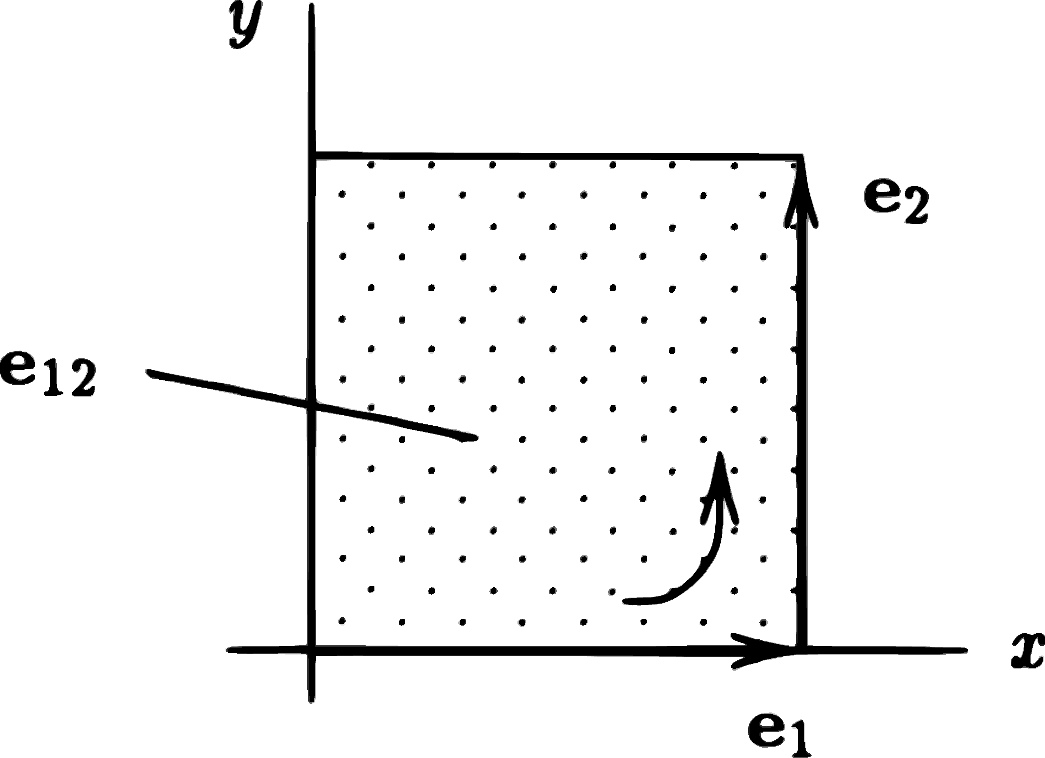
\includegraphics[width=0.4\linewidth]{figures/bivector.pdf}
	\end{center}
	\caption{Representação geométrica de um bivetor $\mathbf{e_{12}}$.}
\end{figure}

\begin{definicao}[Produto de Clifford]
	Sejam dois versores ortogonais $\mathbf{e_1}$ e $\mathbf{e_2}$ no $\mathbb{R}^2$. Para dois vetores $\mathbf{a}$ = $a_1\mathbf{e_1} + a_2\mathbf{e_2}$ e $\mathbf b = b_1\mathbf{e_1} + b_2\mathbf{e_2}$, o \emph{produto de Clifford} $\mathbf{ab}$ é definido como $$\mathbf{ab} = a_1b_1 + a_2b_2 + (a_1b_2-a_2b_1)\mathbf{e_{12}},$$
	isto é, a soma de um escalar com um bivetor.
\end{definicao}



Perceba que pode-se separar as duas partes do produto de Clifford como $$\mathbf{a\cdot b} + \mathbf{a \wedge b} \ = \ a_1b_1 + a_2b_2 + (a_1b_2 - a_2b_1)\mathbf{e_{12}}.$$
\phantomsection
\addcontentsline{toc}{chapter}{Referências Bibliográficas}

\bibliographystyle{unsrt}
\bibliography{references}

\end{document}
